% Chapter 4
\chapter{تعویض مدل‌های شبکه عصبی بین کاربران}

\section{مقدمه}
در فصل پیشین، روش‌های متعددی برای حل مشکل داده‌های
\lr{non-IID}
مورد بررسی قرار گرفتند. در این فصل، رویکرد جامعی برای مقابله با این چالش، یعنی تبادل مدل‌های شبکه عصبی میان کاربران نهایی، بررسی می‌شود که محور اصلی این پایان‌نامه را تشکیل می‌دهد. به منظور درک بهتر، ابتدا یک مثال از داده‌های
\lr{non-IID}
مطرح خواهد شد.

فرض کنید هدف، آموزش مدلی برای تشخیص اشیا مانند علائم ترافیکی و علائم فروشگاهی است. اگر وسایل نقلیه به ترتیب در بزرگراه و مرکز شهر حرکت کنند، داده‌های ویدیویی آن‌ها توزیع‌های متفاوتی از این علائم خواهند داشت. به این معنا که داده‌های آموزشی جمع‌آوری شده از بزرگراه ممکن است کمتر شامل علائم فروشگاهی باشند، در حالی که داده‌های جمع‌آوری شده از مرکز شهر حاوی تعداد بیشتری از هر دو نوع علائم خواهند بود. این تفاوت در توزیع داده‌ها در دستگاه‌های نهایی می‌تواند باعث ایجاد مشکل انحراف وزن‌ها شود.

برای حل این مسئله، عملیات تعویض مدل‌های شبکه عصبی بین کاربران نهایی پیشنهاد می‌شود. این رویکرد، مدل‌ها را بین دستگاه‌های نهایی جابجا می‌کند تا تنوع داده‌ها در دستگاه‌های مختلف کاهش یابد. این عملیات بدون نیاز به هزینه‌های محاسباتی و ارتباطی اضافی، به بهبود عملکرد مدل در مواجهه با داده‌های
\lr{non-IID}
کمک می‌کند.

در این فصل ابتدا ...

\section{
	روش تعویض فدرال%
\LTRfootnote{Federated Swapping}
}

در این روش، یک عملیات جدید به نام تعویض فدرال یا
\lr{FedSwap}
پیشنهاد شده است که جایگزین برخی از دوره‌های
\lr{FedAvg}
در سرور می‌شود. این عملیات با هدف بهبود فرآیند یادگیری فدرال و کاهش تاثیرات منفی داده‌های
\lr{non-IID}
طراحی شده است. اصل اساسی
\lr{FedSwap}
این است که به جای اجرای
\lr{FedAvg}
در هر تکرار، به دستگاه‌های نهایی اجازه می‌دهد تا مدل‌های محلی خود را در سرور با یکدیگر تبادل کنند
\cite{chiu2020semisupervised}.


در روش اصلی یادگیری فدرال، در هر تکرار یک مدل جهانی جدید از ترکیب مدل‌های هر دستگاه نهایی به دست می‌آید. همان‌طور که در شکل
\ref{federated_swapping}
نشان داده شده است، به جای اجرای
\lr{FedAvg}
در هر تکرار، سرور می‌تواند به عنوان یک گزینه دیگر، مدل‌ها را بین دستگاه‌های نهایی تعویض کند. در این روش، به جای اینکه در هر تکرار فرآیند
\lr{FedAvg}
انجام شود، دستگاه‌های نهایی اجازه دارند مدل‌های محلی خود را در سرور با یکدیگر مبادله کنند.


\begin{figure}[b!]
	\centering
	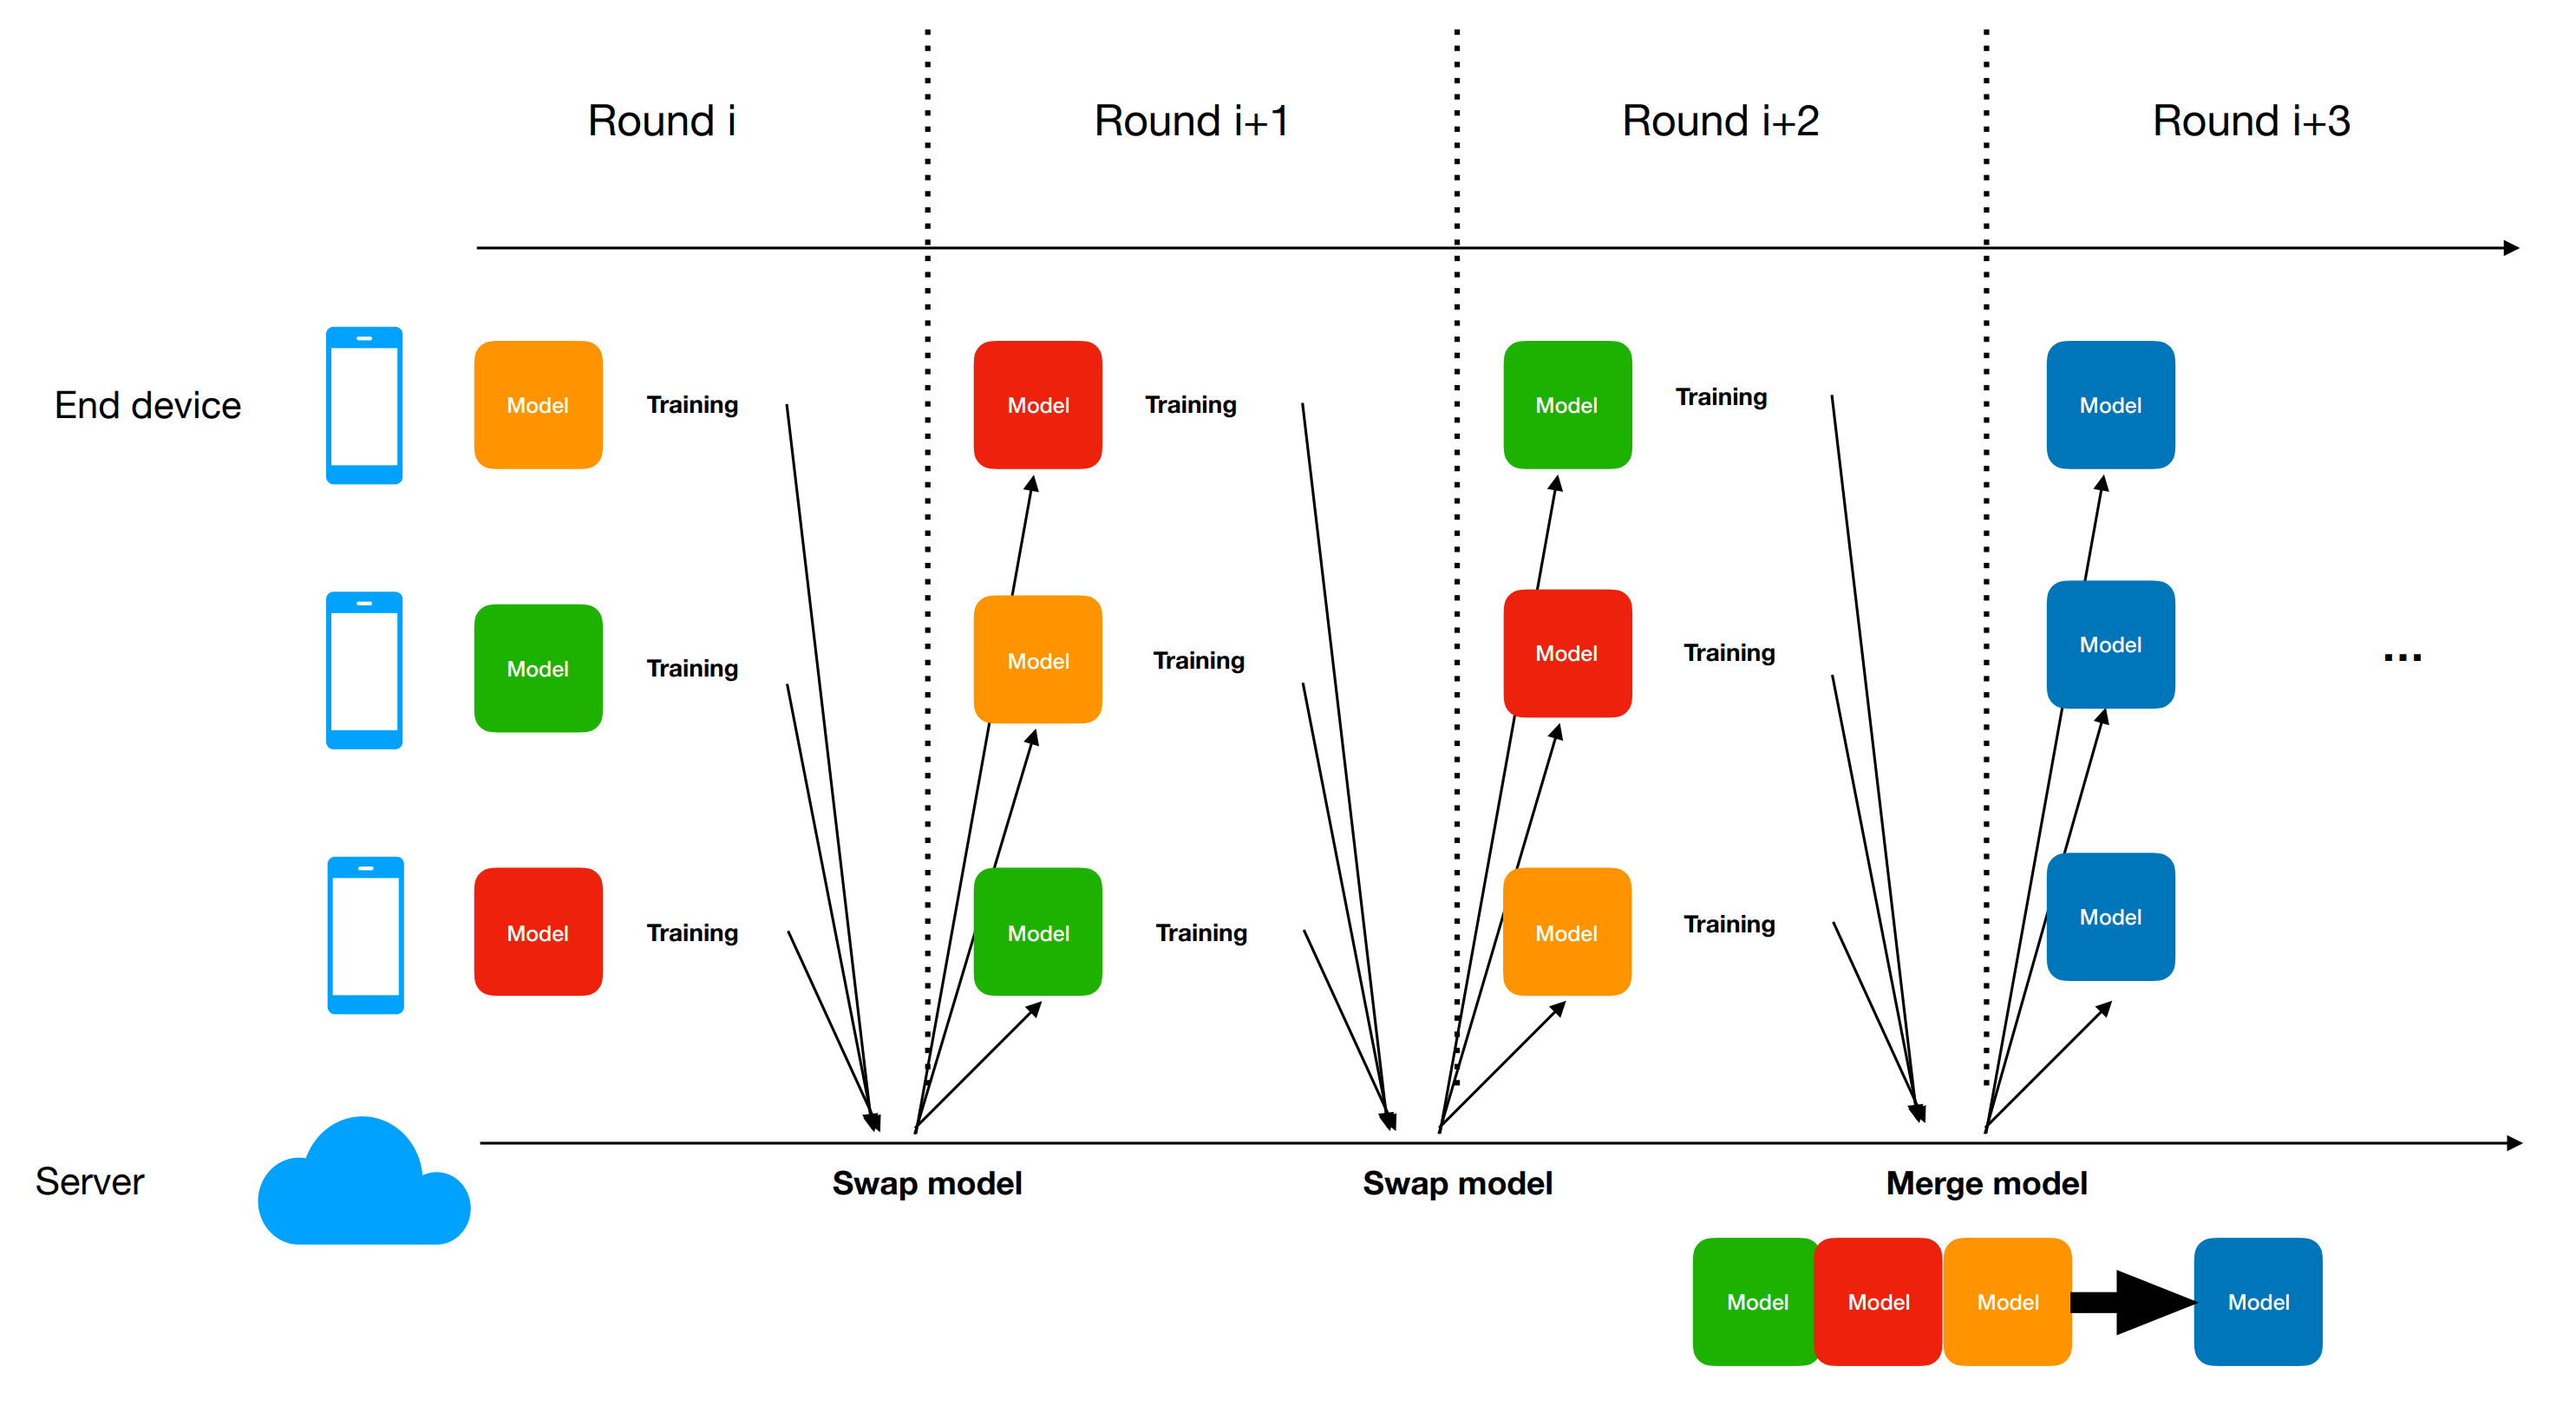
\includegraphics[scale=0.2]{images/chap4/federated_swapping.png}%
	\caption{%
		روش تعویض فدرال
		\cite{chiu2020semisupervised}%
		.
	}
	\label{federated_swapping}
	\centering
\end{figure}


برای حفظ عدالت در این فرآیند، از یک استراتژی چرخشی استفاده می‌شود. در این استراتژی، به طور منظم و به ترتیب، دو دستگاه نهایی به یکدیگر اجازه می‌دهند که مدل‌های خود را تبادل کنند. این کار باعث می‌شود که همه دستگاه‌های نهایی به طور مساوی در فرآیند تبادل مدل‌ها شرکت کنند و هیچ دستگاهی از مزایای این تبادل محروم نماند.

علاوه بر این، انتظار می‌رود که این عملیات تعویض مدل بین دستگاه‌های نهایی، به هر مدل دید گسترده‌تری از کل مجموعه داده‌ها بدهد. به عبارت دیگر، هر مدل محلی با تبادل مدل با دیگر دستگاه‌ها، می‌تواند اطلاعات بیشتری از داده‌های مختلف دریافت کند. این امر به کاهش انحراف وزن‌ها کمک می‌کند، زیرا مدل‌ها با داده‌های متنوع‌تری آموزش می‌بینند و به تدریج به یک مدل جامع‌تر و دقیق‌تر نزدیک می‌شوند.

به طور خلاصه، عملیات
\lr{FedSwap}
با تبادل مدل‌های محلی بین دستگاه‌های نهایی، نه تنها به بهبود دقت و عملکرد مدل‌ها کمک می‌کند، بلکه مشکلات ناشی از داده‌های
\lr{non-IID}
را نیز کاهش می‌دهد. این روش به عنوان یک رویکرد موثر در یادگیری فدرال می‌تواند باعث بهبود قابل توجهی در نتایج نهایی شود
\cite{chiu2020semisupervised}.


جزئیات عملیات
\lr{FedSwap}
در الگوریتم
\ref{algo_FedSwap}
ارائه شده است.
همچنین در جدول
\ref{tabel_FedSwapNotations}
نمادهای مختص این الگوریتم به نمایش در آمده است.
در این الگوریتم،
$w^k_t$
به عنوان وزن مدل در دستگاه نهایی
$k$
پس از گام
$t$
تنظیم می‌شود. در ابتدا، دستگاه‌های نهایی چندین به‌روزرسانی محلی انجام می‌دهند تا مدل‌های خود را بهبود بخشند. پس از هر
$h_1$
به‌روزرسانی محلی، سرور وارد عمل شده و عملیات
\lr{FedSwap}
را اجرا می‌کند. در این مرحله، مدل‌های محلی بین دستگاه‌های نهایی تبادل می‌شوند تا هر دستگاه بتواند از مدل‌های متنوع‌تری برای آموزش استفاده کند.

این تبادل مدل‌ها به کاهش تنوع داده‌ها بین دستگاه‌های مختلف کمک می‌کند و باعث می‌شود که مدل‌ها با داده‌های مختلفی آموزش ببینند. پس از انجام
$h_2$
عملیات
\lr{FedSwap}%
، سرور وارد عمل شده و عملیات
\lr{FedAvg}
را اجرا می‌کند. در این مرحله، سرور مدل‌های محلی را تجمیع می‌کند تا یک مدل مشترک ایجاد شود که از داده‌های تمام دستگاه‌ها بهره‌مند است.


\begin{LTR}
	\SetAlgoNlRelativeSize{-1}
	\begin{algorithm}[t]
		\begin{RTL}
			\caption{%
				تعویض فدرال
				\lr{(FedSwap)}
				\cite{chiu2020semisupervised}
			}
			\label{algo_FedSwap}
		\end{RTL}
		
		\begin{latin}
			Initialize all clients model with weight $w_0$\;
			\For{$t = 1, 2, \ldots, T$}{
				\For{each client $k = 1, 2, \ldots, K$
					\textbf{in parallel}}{
					$w_t^k = w_{t-1}^k - \eta \nabla F(w_{t-1}^k)$\;
				}
				\If{$t|h_1 = 0$ \quad and \quad $t|h_1h_2 \neq 0$}{
					\For{each client $k = 1, 2, \ldots, K$}{
						$w_t^k \gets \texttt{FedSwap}(k, \{w_t^k\}_{k \in K})$\;
					}
				}
				\If{$t|h_1h_2 = 0$}{
					$w_t \gets \texttt{FedAvg}(\{w_t^k\}_{k \in K})$\;
					\For{each client $k = 1, 2, \ldots, K$
						\textbf{in parallel}}{
						$w_t^k \gets w_t$\;
					}
				}
			}
			\SetKwFunction{FedSwap}{FedSwap}
			\SetKwFunction{FedAvg}{FedAvg}
			\SetKwProg{Fn}{Function}{:}{end}
			\Fn{\FedSwap{$k, \{w_t^k\}_{k \in K}$}}{
				$r$ \space represent a random client in \space $K$\;
				$w_t \gets w_t^r$\;
				$w_t^r \gets w_t^k$\;
				\KwRet $w_t$\;
			}
			\Fn{\FedAvg{$\{w_t^k\}_{k \in K}$}}{
				$w_t \gets \sum_{k=1}^K \frac{n_k}{n} w_t^k$\;
				\KwRet $w_t$\;
			}
		\end{latin}
	\end{algorithm}
\end{LTR}


\begin{table}[h]
	\centering
	\caption{نمادهای مختص الگوریتم
		\lr{FedSwap}
	}
	\label{tabel_FedSwapNotations}
	\begin{tabular}{cr}
		\hline
		متغیر & توضیحات \\
		\hline
		$h_1$ & تعداد گام‌ها بین هر
		\lr{FedSwap} \\
		$h_2$ & تعداد
		\lr{FedSwap}
		بین هر
		\lr{FedAvg} \\
		\hline
	\end{tabular}
\end{table}


برای تعیین مقادیر
$h_1$
و
$h_2$%
، ابتدا آزمایش‌های مختلفی انجام شده و بر اساس نتایج به دست آمده، بهینه‌ترین مقادیر انتخاب شده‌اند. در این آزمایش‌ها، چند نکته مهم مشاهده شده است. ابتدا، مقدار
$h_1$
به عملکرد به‌روزرسانی مدل محلی در دستگاه‌های نهایی وابسته است. از آنجایی که وظیفه یادگیری معمولاً یک وظیفه عمومی مثل طبقه‌بندی است، مقدار
$h_1$
بر اساس مقدار گام تعریف‌شده در روش میانگین‌گیری فدرال سنتی تنظیم می‌شود
\cite{chiu2020semisupervised}.

علاوه بر این، مقدار
$h_2$
نقش مهمی در توازن بین سربار ارتباطی و همگرایی مدل ایفا می‌کند. با افزایش مقدار
$h_2$%
، تعداد دفعات تعویض فدرال بین دستگاه‌های نهایی بیشتر خواهد شد. این امر می‌تواند با کاهش تعداد دفعات ادغام فدرال، پهنای باند ارتباطی بیشتری را صرفه‌جویی کند. با این حال، این امر ممکن است باعث افزایش احتمال انحراف وزن‌ها و کاهش دقت همگرایی مدل جهانی شود. به عبارت دیگر، هرچه مقدار
$h_2$
بزرگتر باشد، تعداد دفعاتی که مدل‌ها بین دستگاه‌های نهایی تعویض می‌شوند بیشتر است و این ممکن است به بهبود عملکرد مدل‌ها در مواجهه با داده‌های
\lr{non-IID}
کمک کند، اما ریسک انحراف وزن‌ها نیز بیشتر خواهد شد.

از سوی دیگر، اگر مقدار
$h_2$
کوچکتر باشد، فراوانی تعویض فدرال بین دستگاه‌های نهایی کاهش می‌یابد. این امر منجر به افزایش سربارهای ارتباطی می‌شود زیرا نیاز به ادغام مکرر مدل جهانی خواهد بود. بنابراین، مقدار
$h_2$
باید به گونه‌ای تنظیم شود که توازن مناسبی بین کاهش سربار ارتباطی و حفظ دقت مدل ایجاد کند.

در مجموع، روش
\lr{FedSwap}
با تعویض مدل‌های محلی بین دستگاه‌های نهایی بدون نیاز به هزینه‌های محاسباتی و ارتباطی اضافی، می‌تواند به بهبود عملکرد مدل‌ها در مواجهه با داده‌های
\lr{non-IID}
کمک کند
\cite{chiu2020semisupervised}.



\section{نحوه جابجایی مدل‌ها}
\subsection{جابجایی تصادفی}
در الگوریتم
\lr{FedSwap}%
، مدل‌ها بین دستگاه‌های نهایی جابجا می‌شوند. انتخاب دستگاه‌های نهایی جهت جابجایی به صورت کاملاً تصادفی انجام می‌گیرد، به این معنا که هنگامی که دو دستگاه می‌خواهند مدل‌های خود را جابجا کنند، فرآیند انتخاب این دو دستگاه به صورت کاملاً تصادفی انجام می‌شود. این تصادفی بودن انتخاب دستگاه‌ها باعث می‌شود که هیچ الگوی ثابتی در جابجایی مدل‌ها وجود نداشته باشد و هر بار ترکیب جدیدی از دستگاه‌ها در فرآیند تبادل مدل شرکت کنند.

یکی از ویژگی‌های مهم الگوریتم
\lr{FedSwap}
این است که تمام دستگاه‌های نهایی به صورت مساوی و عادلانه در این فرآیند جابجایی شرکت می‌کنند. به عبارت دیگر، همه دستگاه‌ها بدون استثنا در فرآیند جابجایی قرار می‌گیرند، اما انتخاب دستگاه‌ها برای جابجایی به صورت تصادفی صورت می‌پذیرد. این روش باعث می‌شود که تمامی دستگاه‌ها فرصت مساوی برای تبادل مدل‌ها و بهبود دقت و عملکرد خود داشته باشند.

با استفاده از این رویکرد، الگوریتم
\lr{FedSwap}
قادر است به بهبود عملکرد مدل‌های محلی کمک کند، زیرا تبادل تصادفی مدل‌ها بین دستگاه‌ها باعث می‌شود که هر دستگاه به داده‌ها و اطلاعات بیشتری دسترسی پیدا کند. این امر به کاهش انحراف وزن‌ها و بهبود همگرایی مدل جهانی کمک می‌کند.


\subsection{جابجایی بر اساس میزان مشابهت مدل‌ها}
در این پژوهش، هدف اصلی انتخاب دستگاه‌های نهایی بر اساس میزان شباهت مدل‌های شبکه عصبی و جابجایی آن‌ها با یکدیگر است. برای این منظور، باید به طور کامل با ساختار شبکه عصبی آشنا بوده و مدل‌های مختلف را با یکدیگر مقایسه کرد. این مقایسه به ما کمک می‌کند تا میزان شباهت و تفاوت بین مدل‌های شبکه عصبی دستگاه‌های نهایی را ارزیابی کنیم.

بعد از بررسی و تعیین میزان شباهت مدل‌ها، باید تصمیم گرفت که کدام یک از آن‌ها را با یکدیگر جابجا کنیم. بهترین انتخاب برای جابجایی، مدلی است که کمترین شباهت را با مدل شبکه عصبی دستگاه فعلی دارد. دلیل این انتخاب این است که اگر مدل دستگاه فعلی با مدل دستگاه مقصد شباهت زیادی داشته باشد، جابجایی آن‌ها مؤثر نخواهد بود. این شباهت بالا به این معناست که این دو دستگاه نهایی داده‌های مشابهی داشته و در طول زمان آموزش‌های مشابهی دیده‌اند، بنابراین جابجایی مدل‌ها تأثیر قابل‌توجهی بر بهبود یادگیری نخواهد داشت.

بنابراین، انتخاب مدل‌هایی با کمترین شباهت بین دستگاه‌های نهایی می‌تواند به بهبود فرآیند یادگیری کمک کند. این فرض بر این اساس است که دستگاه‌هایی با مدل‌های متفاوت احتمالاً داده‌هایی با ساختارهای متفاوت دارند. جابجایی مدل‌ها بین این دستگاه‌ها، مدل‌ها را با داده‌های جدیدی روبه‌رو می‌کند که می‌تواند به یادگیری بهتر و متنوع‌تر کمک کند. در نتیجه، مدل سراسری سریع‌تر به سمت مسیر بهینه همگرا می‌شود و دقت و کارایی آن افزایش می‌یابد.

این روش نه تنها تنوع داده‌ها را در فرآیند یادگیری افزایش می‌دهد، بلکه به کاهش انحراف وزن‌ها نیز کمک می‌کند. با داشتن دید گسترده‌تری از داده‌ها و تجربیات مختلف، مدل‌ها می‌توانند بهتر و جامع‌تر آموزش ببینند. این امر در نهایت منجر به بهبود عملکرد کلی مدل در شرایط واقعی می‌شود و کمک می‌کند که مدل‌های یادگیری فدرال بتوانند با چالش‌های داده‌های
\lr{non-IID}
به نحو بهتری مقابله کنند.

\subsection{بار محاسباتی جهت بررسی مشابهت}

در این روش، ابتدا تمام مدل‌های شبکه عصبی از دستگاه‌های نهایی به سمت سرور ارسال می‌شوند. سپس سرور بر اساس معیارهای مشخصی، شباهت بین این مدل‌ها را بررسی و اقدام به جابجایی آن‌ها می‌کند. در این فرآیند، تمامی محاسبات پردازشی در سرور انجام می‌شود.

افزایش بار کاری در سرور از نظر محاسباتی مشکلی ایجاد نمی‌کند زیرا سرور به‌طور خاص برای انجام چنین عملیات‌هایی طراحی شده است. در یادگیری فدرال، فرض بر این است که دستگاه‌های نهایی دارای سخت‌افزار ضعیف و منابع محدود هستند، بنابراین بار محاسباتی سنگین بر عهده آن‌ها گذاشته نمی‌شود. در این روش نیز تمامی پردازش‌های سنگین بر روی سرور انجام می‌شود که از قدرت پردازشی بالایی برخوردار است و می‌تواند به راحتی این عملیات را مدیریت کند.

سرورهای مرکزی معمولاً دارای منابع پردازشی قوی، حافظه زیاد و قابلیت‌های پیشرفته برای انجام محاسبات پیچیده هستند. این ویژگی‌ها به سرور اجازه می‌دهد تا بدون هیچ مشکلی عملیات‌هایی مانند تعویض مدل‌ها و تجمیع نتایج را انجام دهد. این امر به خصوص در مورد یادگیری فدرال بسیار حیاتی است زیرا بار محاسباتی سنگین نباید بر دستگاه‌های نهایی با سخت‌افزار ضعیف تحمیل شود.

با انجام عملیات بر روی سرور، دستگاه‌های نهایی تنها به تبادل داده‌های لازم و اجرای به‌روزرسانی‌های محلی سبک می‌پردازند. این رویکرد باعث خواهد شد که فرآیند یادگیری بهینه‌تری ایجاد شود و مدل‌ها به طور موثر و کارآمدتری آموزش ببینند. در نتیجه، مشکلات محاسباتی به حداقل می‌رسد و عملکرد کلی سیستم بهبود خواهد یافت.

این روش نه تنها به حفظ منابع محدود دستگاه‌های نهایی کمک می‌کند، بلکه بهره‌وری بالاتری نیز از قدرت پردازشی سرور به دست می‌آید. به این ترتیب، می‌توان اطمینان داشت که عملیات‌های پیچیده و محاسبات سنگین به درستی و با سرعت مناسب انجام می‌شوند، بدون اینکه فشار اضافی بر دستگاه‌های نهایی وارد شود. به این ترتیب، این روش می‌تواند به طور موثری در محیط‌های مختلف با دستگاه‌های متنوع و منابع محدود پیاده‌سازی شود و نتایج قابل اعتمادی ارائه دهد.


\section{معیارهای مشابهت}
\subsection{تعریف مسئله}
فرض کنید \( X \) ماتریسی با ابعاد \( n \times p_1 \) باشد که \( X \in \mathbb{R}^{n \times p_1} \) شامل \( n \) نمونه و \( p_1 \) ویژگی است. همچنین، \( Y \) ماتریسی با ابعاد \( n \times p_2 \) باشد که \( Y \in \mathbb{R}^{n \times p_2} \) شامل \( n \) نمونه و \( p_2 \) ویژگی است. فرض می‌شود که \( p_1 \) کمتر یا مساوی \( p_2 \) است.

هدف طراحی و تحلیل یک شاخص شباهت عددی \( s(X, Y) \) است که بتواند بازنمایی‌های%
\LTRfootnote{Representations}
موجود در ماتریس‌های \( X \) و \( Y \) را هم درون یک شبکه عصبی و هم بین شبکه‌های عصبی مختلف مقایسه کند. چنین شاخصی به ما کمک می‌کند تا تاثیر عوامل مختلف در یادگیری عمیق را بهتر درک کرده و این تاثیرات را به تصویر بکشیم.

به عنوان مثال، در بررسی شبکه‌های عصبی، ماتریس \( X \) می‌تواند نمایانگر فعال‌سازهای%
\LTRfootnote{Activations}
نورون‌ها در یک لایه خاص برای \( n \) نمونه ورودی باشد و ماتریس \( Y \) می‌تواند نمایانگر فعال‌سازهای نورون‌ها در لایه‌ای دیگر یا حتی در یک شبکه عصبی دیگر برای همان \( n \) نمونه باشد. مقایسه این دو ماتریس اطلاعات مهمی درباره نحوه یادگیری و بازنمایی داده‌ها توسط شبکه عصبی ارائه می‌دهد.

شاخص \( s(X, Y) \) باید توانایی اندازه‌گیری شباهت‌ها و تفاوت‌های بین بازنمایی‌های مختلف را داشته باشد. این شاخص می‌تواند به پژوهشگران کمک کند تا نحوه تغییر بازنمایی‌ها در اثر عوامل مختلف مانند تغییرات در داده‌های ورودی، تغییرات در معماری شبکه یا تغییرات در پارامترهای آموزش را بهتر درک کنند.

طراحی و تحلیل این شاخص شباهت می‌تواند به بهبود فهم ما از نحوه عملکرد شبکه‌های عصبی کمک کند و ابزار مفیدی برای بهبود روش‌های آموزش و بهینه‌سازی شبکه‌های عصبی فراهم کند.


\section{معیار مشابهت در چه مواردی می‌بایست پایدار باشد}
این بخش ویژگی‌های لازم برای یک معیار مقایسه بازنمایی‌های شبکه عصبی را بررسی می‌کند. این بررسی شامل تحلیل پایداری شاخص‌های شباهت و تأثیرات آن‌ها در اندازه‌گیری شباهت بازنمایی‌های شبکه عصبی است. اهمیت این موضوع در این است که معیار شباهت مورد استفاده باید نسبت به تبدیل متعامد%
\LTRfootnote{Orthogonal Transformation}
و مقیاس‌بندی همسان‌گرد%
\LTRfootnote{Isotropic Scaling}
پایدار باشد. این ویژگی‌ها به معیار شباهت امکان می‌دهند تا بازنمایی‌های شبکه عصبی را به درستی مقایسه کرده و تأثیرات مختلف در فرآیند آموزش شبکه عصبی را بهتر درک کند.


\subsection{تبدیل متعامد}

پایداری نسبت به تبدیل‌های متعامد به این معناست که اگر \( s(X, Y) \) یک شاخص شباهت بین دو ماتریس \( X \) و \( Y \) باشد، این شاخص باید در مقابل تغییرات متعامد نیز پایدار باقی بماند. به عبارت دیگر، اگر \( U \) و \( V \) ماتریس‌های متعامد با رتبه کامل%
\LTRfootnote{Full Rank}
باشند که \( U^TU = I \) و \( V^TV = I \) را برآورده کنند، باید \( s(X, Y) = s(XU, YV) \) باشد. این ویژگی تضمین می‌کند که حتی در صورتی که ابعاد \( p \) بزرگتر از \( n \) باشند، شاخص شباهت همچنان به‌طور مطلوب عمل می‌کند. علاوه بر این، تبدیل‌های متعامد خواص مهمی از جمله حفظ حاصل‌ضرب‌های عددی و فاصله‌های اقلیدسی%
\LTRfootnote{Euclidean Distances}
بین نمونه‌ها را نیز حفظ می‌کنند. این امر باعث می‌شود که مقایسه‌های انجام شده توسط این شاخص‌ها دقیق و قابل اعتماد باشند
\cite{kornblith2019similarity}.

پایداری نسبت به تبدیل‌های متعامد برای شبکه‌های عصبی که با استفاده از روش نزول گرادیان آموزش داده می‌شوند، بسیار مطلوب است. این ویژگی نه تنها پایداری نسبت به تغییرات متعامد را تضمین می‌کند بلکه شامل پایداری نسبت به جایگشت نیز می‌شود. جایگشت در یک ماتریس به معنای این است که مقدارهای درون ماتریس فقط جابجا می‌شوند و ارزش‌های آن‌ها ثابت باقی می‌مانند. این پایداری برای تطبیق تقارن‌های شبکه‌های عصبی ضروری است
\cite{chen1993geometry, orhan2017skip}.

در حالت خطی، اگر ورودی‌ها با یک تبدیل متعامد تغییر کنند، روند آموزش با روش نزول گرادیان تحت تأثیر قرار نمی‌گیرد. برای شبکه‌های عصبی که با وزن‌های متقارن و تصادفی شروع می‌شوند، تبدیل‌های متعامد بر فعال‌سازها باعث می‌شود که روند آموزشی مشابه حالت بدون تغییر باقی بماند. اما اگر یک تغییر خطی دلخواه انجام شود، این ویژگی حفظ نمی‌شود و ممکن است روند آموزش تحت تأثیر منفی قرار گیرد
\cite{lecun1990second}.

به‌طور کلی، پایداری نسبت به تبدیل‌های متعامد در شبکه‌های عصبی اهمیت زیادی دارد زیرا این ویژگی کمک می‌کند تا شبکه‌های عصبی در مواجهه با تغییرات متقارن در داده‌ها، به درستی عمل کنند و دقت و کارایی آن‌ها در فرآیند آموزش بهینه باقی بماند.



\subsection{مقیاس‌بندی همسان‌گرد}
انتظار می‌رود که شاخص‌های شباهت زمانی که ورودی‌ها به صورت همسان مقیاس‌بندی می‌شوند، پایدار بمانند. به این معنا که اگر ورودی‌ها با ضرایب مثبت \(\alpha\) و \(\beta\) ضرب شوند، شاخص شباهت نباید تغییری کند. به عبارتی دیگر، \( s(X, Y) = s(\alpha X, \beta Y) \) باید برای هر \(\alpha\) و \(\beta\) مثبت صحیح باشد.

این ویژگی اهمیت خاصی دارد زیرا تضمین می‌کند که مقایسه بازنمایی‌های شبکه‌های عصبی تحت تأثیر مقیاس‌بندی یکسان قرار نمی‌گیرد و دقت شاخص حفظ می‌شود. در واقع، این شاخص‌ها قادرند در شرایطی که شبکه‌های عصبی تحت تغییرات یکسان مقیاس قرار می‌گیرند، همچنان به درستی بازنمایی‌های مختلف را مقایسه کنند. 

از سوی دیگر، شاخص‌هایی که در برابر مقیاس‌بندی همسان‌گرد پایدار هستند، اما نسبت به مقیاس‌بندی غیرهمسان‌گرد (یعنی تغییر مقیاس ویژگی‌های فردی) مقاوم نیستند، اهمیت ویژه‌ای دارند. این شاخص‌ها می‌توانند به دقت بیشتری در مقایسه بازنمایی‌های شبکه‌های عصبی کمک کنند و به درک بهتر تأثیرات مختلف در فرآیند یادگیری عمیق یاری رسانند
\cite{kornblith2019similarity}.

به عنوان مثال، وقتی شبکه‌های عصبی در معرض تغییرات یکسان مقیاس قرار می‌گیرند، این شاخص‌ها همچنان قادر خواهند بود بازنمایی‌های مختلف را به درستی مقایسه کنند. این ویژگی امکان فهم بهتر تأثیرات گوناگون در طول آموزش شبکه‌های عصبی و استفاده از این شاخص‌ها برای تحلیل و بهبود عملکرد مدل‌ها را فراهم می‌کند. بنابراین، شاخص‌های مقاوم در برابر مقیاس‌بندی همسان‌گرد می‌توانند ابزار مفیدی برای ارزیابی و بهینه‌سازی شبکه‌های عصبی باشند.



\section{مقایسه ساختارهای مشابهت}
در تحلیل بازنمایی‌های شبکه‌های عصبی، یکی از چالش‌های اصلی مقایسه ویژگی‌های چندگانه هر نمونه در بازنمایی‌های مختلف است. این روش ممکن است پیچیده و زمان‌بر باشد و نتایج گمراه‌کننده‌ای ایجاد کند. برای حل این مشکل، می‌توان از رویکردی استفاده کرد که به جای مقایسه مستقیم ویژگی‌های هر نمونه، ساختارهای شباهتی بین نمونه‌ها را بررسی کند.

ایده اصلی این است که به جای مقایسه مستقیم ویژگی‌های چندگانه هر نمونه در دو بازنمایی مختلف، می‌توان ابتدا شباهت بین هر جفت نمونه در هر بازنمایی را به صورت جداگانه سنجید و سپس این ساختارهای شباهتی را با هم مقایسه کرد
\cite{kornblith2019similarity}.

برای روشن‌تر شدن این موضوع، فرض کنید به جای اینکه به صورت مستقیم ویژگی‌های چند بعدی دو نمونه را با هم مقایسه کنیم، ابتدا بررسی می‌کنیم که هر کدام از این نمونه‌ها چقدر به سایر نمونه‌ها شباهت دارند. سپس این ماتریس‌های شباهت بازنمایی را که هر کدام نشان‌دهنده میزان شباهت یک نمونه به سایر نمونه‌ها است، با هم مقایسه می‌کنیم.

نکته مهم این است که اگر برای اندازه‌گیری شباهت از ضرب داخلی استفاده شود، شباهت بین ماتریس‌های بازنمایی به یک مفهوم دیگر و قابل درک از شباهت بین ویژگی‌های جفتی تبدیل می‌شود. به عبارت دیگر، این روش امکان دست‌یابی به درک دقیق‌تری از شباهت بین ویژگی‌ها را بدون مقایسه مستقیم ویژگی‌های چندگانه هر نمونه فراهم می‌کند. این رویکرد می‌تواند به طور قابل توجهی در تحلیل و درک بازنمایی‌های شبکه‌های عصبی و داده‌های پیچیده مؤثر باشد، زیرا ساختارهای پیچیده را به شیوه‌ای ساده‌تر و قابل فهم‌تر بررسی می‌کند.



\subsection{
	انتخاب هسته%
	\LTRfootnote{Kernel}
}
در معیارهای مشابهت و اندازه‌گیری وابستگی، مفهوم هسته یا
\lr{kernel}
نقش بسیار مهمی دارد. هسته در واقع یک تابع ریاضی است که برای محاسبه شباهت بین داده‌های ورودی استفاده می‌شود. این تابع، داده‌ها را به یک فضای ویژگی بالاتر نگاشت می‌کند تا بتوان همبستگی‌ها و مشابهت‌های پیچیده‌تر بین آن‌ها را بهتر سنجید.

به بیان ساده‌تر، تابع هسته \( k \) یک تابع مثبت معین است که دو بردار ورودی \( x_i \) و \( x_j \) را گرفته و یک عدد حقیقی تولید می‌کند که نشان‌دهنده میزان شباهت بین این دو بردار است. هسته‌ها می‌توانند به شکل‌های مختلفی باشند که هر کدام ویژگی‌ها و کاربردهای خاص خود را دارند. در اینجا به چند نمونه رایج اشاره می‌شود.

\begin{itemize}
\item
هسته خطی%
\LTRfootnote{Linear Kernel}:
این هسته به سادگی ضرب داخلی%
\LTRfootnote{Inner Product}
دو بردار ورودی را محاسبه می‌کند.
\begin{equation*}
	k(x_i, x_j) = x_i^T x_j
\end{equation*}
	
	
	
\item 
هسته چندجمله‌ای%
\LTRfootnote{Polynomial Kernel}:
این هسته ضرب داخلی را با یک توان مثبت، بالا می‌برد.
\begin{equation*}
	k(x_i, x_j) = (x_i^T x_j + c)^d
\end{equation*}
که در آن \( c \) یک ثابت و \( d \) درجه چندجمله‌ای است.

	
\item
هسته گاوسی
\lr{(RBF)}%
\LTRfootnote{Radial Basis Function Kernel}:
این هسته فاصله اقلیدسی بین دو بردار را در یک تابع نمایی قرار می‌دهد، که باعث می‌شود داده‌هایی که نزدیک به هم هستند شباهت بیشتری داشته باشند.
\begin{equation*}
	k(x_i, x_j) = \exp\left(-\frac{||x_i - x_j||^2}{2\sigma^2}\right)
\end{equation*}
که در آن \( \sigma \) پارامتر پهنای باند است و تنظیم‌کننده میزان تاثیر فاصله می‌باشد.
\end{itemize}

برای هسته
\lr{RBF}%
، چندین استراتژی مختلف برای انتخاب پهنای باند \(\sigma\) وجود دارد که میزان تأکید بر شباهت فواصل کوچک نسبت به فواصل بزرگ را کنترل می‌کند. \(\sigma\) به عنوان کسری از فاصله میانه بین نمونه‌ها تنظیم می‌شود. در عمل، مشاهده می‌شود که هسته‌های
\lr{RBF}
و خطی در بیشتر آزمایش‌ها نتایج مشابهی ارائه می‌دهند
\cite{kornblith2019similarity}.

استفاده از توابع هسته‌ای در معیارهای مشابهت و وابستگی، این امکان را فراهم می‌کند که داده‌های ورودی به یک فضای ویژگی بالاتر نگاشت شوند، جایی که روابط پیچیده و غیرخطی بین داده‌ها می‌توانند به صورت ساده‌تری مدل‌سازی شوند. به این ترتیب، معیارها با بهره‌گیری از هسته‌ها می‌توانند تحلیل دقیق‌تر و کارآمدتری از داده‌های پیچیده ارائه دهند. این ویژگی باعث می‌شود که هسته‌ها ابزار قدرتمندی در تحلیل داده‌ها باشند.



\subsection{شباهت مبتنی بر ضرب داخلی}
یک فرمول ساده وجود دارد که ضرب داخلی بین نمونه‌ها را با ضرب داخلی بین ویژگی‌ها مرتبط می‌سازد:
\begin{equation}
	\langle \text{vec}(XX^T), \text{vec}(YY^T) \rangle = \text{tr}(XX^TYY^T) = ||Y^TX||_F^2
	\label{eq_DotProduct}
\end{equation}
در فرمول
\eqref{eq_DotProduct}%
، عناصر \(XX^T\) و \(YY^T\) نشان‌دهنده ضرب داخلی بین بازنمایی نمونه‌های \(i\) و \(j\) هستند و شباهت بین این نمونه‌ها را بر اساس شبکه‌های مربوطه نشان می‌دهند. 

به بیان دیگر، بخش چپ فرمول
\eqref{eq_DotProduct}%
، میزان مشابهت بین الگوهای شباهت، میان نمونه‌ها را ارزیابی می‌کند. این در حالی است که سمت راست، با جمع کردن مربعات ضرب‌های داخلی بین هر جفت از نمونه‌ها، به همان نتیجه مشابه می‌رسد و شباهت بین ویژگی‌های \(X\) و \(Y\) را اندازه‌گیری می‌کند.

این فرمول نشان می‌دهد که می‌توان به جای مقایسه مستقیم ویژگی‌ها، از شباهت‌های بین نمونه‌ها استفاده کرد تا به فهم بهتری از بازنمایی‌های شبکه‌های عصبی و داده‌های پیچیده دست یافت. به این ترتیب، تحلیل و درک داده‌ها ساده‌تر و مؤثرتر خواهد بود، زیرا این روش به ما اجازه می‌دهد تا به صورت غیرمستقیم و با استفاده از شباهت‌های موجود بین نمونه‌ها، به نتایج دقیق‌تری برسیم.


\subsection{
	معیار استقلال هیلبرت-اشمیت
	\lr{(HSIC)}%
	\LTRfootnote{Hilbert-Schmidt Independence Criterion}
	}
برای بررسی میزان وابستگی و شباهت بین دو مجموعه داده، می‌توان از معیار استقلال هیلبرت-اشمیت استفاده کرد. این معیار به طور خاص برای اندازه‌گیری همبستگی بین داده‌های مختلف طراحی شده است. به طور دقیق‌تر، برای داده‌های مرکزیت‌یافته (میانگین صفر در هر ستون) \(X\) و \(Y\)، رابطه زیر برقرار است:
\begin{equation*}
	\frac{1}{(n - 1)^2} \text{tr}(XX^TYY^T) = ||\text{cov}(X^T, Y^T)||_F^2
\end{equation*}

معیار
\lr{HSIC}
این معادله را با استفاده از فضایی خاص تعمیم می‌دهد و امکان بررسی مؤثر وابستگی‌ها را فراهم می‌کند. به بیان دیگر، این معیار با بهره‌گیری از توابع هسته‌ای، همبستگی بین ماتریس‌های داده را اندازه‌گیری می‌کند. به این نحو که عناصر \(K_{ij}\) و \(L_{ij}\) به ترتیب از طریق \(k(x_i, x_j)\) و \(l(y_i, y_j)\) محاسبه می‌شوند، که در اینجا \(k\) و \(l\) توابع هسته‌ای هستند
\cite{gretton2005measuring}.

برآورد
\lr{HSIC}
به صورت زیر تعریف می‌شود:
\begin{equation}
	\text{HSIC}(K, L) = \frac{1}{(n - 1)^2} \text{tr}(KHLH)
	\label{eq_HSIC}
\end{equation}
در فرمول
\eqref{eq_HSIC}،
\(H\)
ماتریس مرکزیت‌دهنده است و به شکل \(H_n = I_n - \frac{1}{n} 11^T\) تعریف می‌شود.

نکته جالب اینجاست که اگر هسته‌های خطی \(k\) و \(l\) به صورت \(k(x, y) = l(x, y) = x^Ty\) باشند،
\lr{HSIC}
به همان معادله اولیه برمی‌گردد. این بدین معناست که معیار
\lr{HSIC}
می‌تواند به ما کمک کند تا به شکلی دقیق و قابل اعتماد، میزان وابستگی و شباهت بین داده‌ها را ارزیابی کنیم و درک بهتری از ساختارهای پیچیده داده‌ها به دست آوریم.


\subsection{
	معیار هم‌ترازی هسته مرکزی
	\lr{(CKA)}%
	\LTRfootnote{Centered Kernel Alignment}
}
معیار
\lr{HSIC}
در اندازه‌گیری همبستگی‌ها با مشکل عدم پایداری نسبت به مقیاس‌بندی همسان‌گرد ویژگی‌ها مواجه است. این بدان معناست که در صورت تغییر مقیاس ویژگی‌ها، نتیجه
\lr{HSIC}
ممکن است دستخوش تغییراتی شود که به درستی شباهت‌های بین داده‌ها را نشان ندهد. برای رفع این مورد، از فرم نرمال‌شده‌ای به نام هم‌ترازی هسته مرکزی استفاده می‌شود.

\lr{CKA}
یک شاخص نرمال‌شده است که تأثیر مقیاس‌بندی همسان‌گرد را حذف می‌کند و به این ترتیب، دقت و پایداری بیشتری در مقایسه بازنمایی‌های شبکه‌های عصبی فراهم می‌آورد
\cite{cortes2012algorithms, cristianini2001kernel}.
فرمول
\lr{CKA}
به شکل زیر تعریف می‌شود:
\begin{equation}
	\text{CKA}(K, L) = \frac{\text{HSIC}(K, L)}{\sqrt{\text{HSIC}(K, K) \cdot \text{HSIC}(L, L)}}
	\label{eq_CKA}
\end{equation}
در فرمول
\eqref{eq_CKA}،
عبارت \(\text{HSIC}(K, L)\) میزان همبستگی بین دو ماتریس هسته‌ای \(K\) و \(L\) را اندازه‌گیری می‌کند. صورت کسر، همان
\lr{HSIC}
اصلی است که میزان همبستگی بین دو ماتریس داده را نشان می‌دهد. اما برای نرمال‌سازی این مقدار و حذف تأثیر مقیاس‌بندی، مخرج کسر به کار می‌رود که شامل ضرب دو
\lr{HSIC}
مربوط به هر یک از ماتریس‌ها با خودشان است. این نرمال‌سازی باعث می‌شود که نتیجه نهایی مستقل از مقیاس‌بندی ویژگی‌ها باشد و شباهت‌های واقعی بین داده‌ها را بهتر منعکس کند.

استفاده از
\lr{CKA}
در مقایسه با
\lr{HSIC}%
، به‌ویژه در تحلیل بازنمایی‌های شبکه‌های عصبی و داده‌های پیچیده، کارایی بهتری دارد. زیرا این شاخص نرمال‌شده، نه تنها شباهت‌های بین داده‌ها را دقیق‌تر می‌سنجد، بلکه در برابر تغییرات مقیاس‌بندی نیز مقاوم است. به این ترتیب، می‌توان از
\lr{CKA}
به عنوان یک ابزار قدرتمند برای درک و تحلیل بازنمایی‌های مختلف در یادگیری عمیق و دیگر زمینه‌های مرتبط استفاده کرد.


\section{روش‌های سنجش شباهت در بازنمایی‌های شبکه عصبی}
در این بخش به بررسی روش‌های مختلفی که برای سنجش شباهت بین بازنمایی‌های شبکه‌های عصبی استفاده می‌شود، پرداخته خواهد شد. یکی از روش‌های مهم در این زمینه استفاده از پایه‌های متعامد است. به طور خاص، فرض می‌کنیم که \( Q_X \) و \( Q_Y \) پایه‌های متعامدی برای ستون‌های ماتریس‌های \( X \) و \( Y \) هستند. به این معنا که \( Q_X \) و \( Q_Y \) به صورت \( Q_X = X(X^T X)^{-1/2} \) و \( Q_Y = Y(Y^T Y)^{-1/2} \) تعریف شده‌اند. این پایه‌های متعامد به ما اجازه می‌دهند تا بازنمایی‌های شبکه عصبی را به صورت موثرتری تحلیل کنیم و شباهت‌های آن‌ها را با دقت بیشتری بسنجیم.

استفاده از پایه‌های متعامد به این معنی است که ما می‌توانیم بدون نگرانی از وابستگی‌های خطی بین ستون‌ها، شباهت‌ها را به صورت مستقیم مقایسه کنیم. این رویکرد به ویژه زمانی مفید است که می‌خواهیم درک کنیم چگونه شبکه عصبی ویژگی‌های مختلف داده‌ها را استخراج و بازنمایی می‌کند. با این روش می‌توانیم تحلیل‌های دقیقی انجام دهیم و بفهمیم که چگونه تغییرات در داده‌های ورودی یا ساختار شبکه، بازنمایی‌های داخلی شبکه را تحت تاثیر قرار می‌دهند. این نوع تحلیل‌ها می‌تواند به بهبود و بهینه‌سازی شبکه‌های عصبی و الگوریتم‌های یادگیری عمیق کمک شایانی کند.


\subsection{sum\_diff}
تست

\subsection{CCA}
تست

\subsection{dCKA}
تست


\subsection{نحوه پیداکردن مشابهت، لایه به لایه}
تست

\section{نحوه جستجوی کاربر نهایی جهت جابجایی مدل}
تست

\subsection{روش بهینه}
تست

\subsection{روش حریصانه}
تست






